\begin{abstract}
Wearable irregular time series vary simultaneously in sensor value scale,
observation support, and within-patch waveform. Pooling these factors into one
patch token can preserve local level while erasing ordered motion, or preserve
motion while mixing unsupported temporal ranges. We introduce the
Multiresolution Evidence Separation and Anchoring Network (MESANet), an
end-to-end forecasting backbone that represents every variable through two
complementary coordinates. A masked affine anchor canonicalizes each observed
history and restores its physical coordinate after prediction. A
multiresolution support branch forms a bounded low-frequency coordinate, while an
ordered waveform branch encodes masked values, observation patterns, and first
differences without pooling away patch order. The coordinates produce a
low-rank cosine forecast and a direct trajectory; fixed low-frequency
subtraction with coefficient $\rho=0.5$ bounds overlap before summation. The analysis
characterizes conditional affine equivariance, collisions induced by pooled
patch statistics, and dual-coordinate excess risk through low-frequency
approximation, waveform residual, and subspace overlap. On six wearable
datasets, one public comparator per dataset is frozen by validation error
before five-run test evaluation. MESANet obtains lower mean error in 9 of 12
mean squared error (MSE) and mean absolute error (MAE) cells and on both metrics
for four datasets; six cells have paired bootstrap intervals over optimization
runs favoring MESANet. Parameter-matched controls
support the dual-coordinate factorization, multiresolution support, and ordered
discrete cosine transform (DCT) basis, while showing that waveform and
affine-anchor contributions are regime dependent. HumanActivity MSE and
USC-HAD delimit the empirical scope.
\end{abstract}

\section{Introduction}

Irregular multivariate time-series (IMTS) forecasting predicts future values
from asynchronous and partially observed histories. Continuous-time dynamics,
time-aware attention, graph propagation, and adaptive patching make timestamps
and missingness visible to the predictor~\citep{rubanova2019latent,
shukla2021mtan,cru2022,raindrop2022,grafiti2024,tpatchgnn2024,apn2026,
kafnet2026}. Wearable streams add structured variation: sensor offsets and
amplitudes change across users and sessions, sensor groups are not always
co-observed, and short motion transients coexist with slower postural trends.
An effective wearable forecaster must therefore preserve the physical sensor
coordinate, observation support, and ordered waveform simultaneously.

Patch forecasting compresses observations into a finite set of tokens, but one
token is often asked to perform incompatible roles. A wider or adaptively
selected support can stabilize a sparse patch, yet averaging that support can
erase within-patch order. Conversely, a short ordered patch preserves motion
but may lack enough evidence under stale or asynchronous sampling. Figure
\ref{fig:mesa-motivation} illustrates the support side of this conflict: the
predictive temporal range changes across local observation states, so neither
one selected range nor unconditional scale mixing is uniformly reliable. The
same compression can also create waveform collisions: increasing and decreasing
segments can share their mean, variance, density, and endpoints after pooling
while implying different futures.

\begin{figure}[t]
\centering
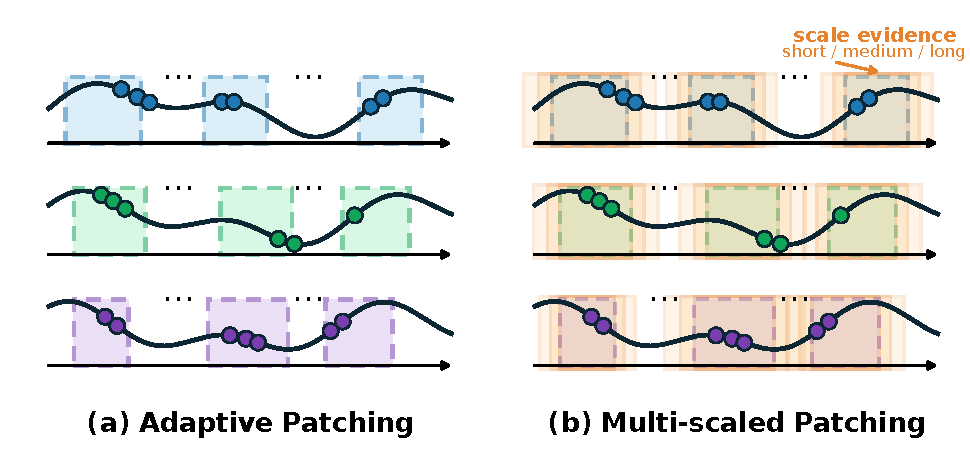
\includegraphics[width=\columnwidth]{figures/final/mesa_fig1_apn_like_v540.pdf}
\caption{Single-support adaptive patching and multiscale patch evidence.
Irregular density and recency change the useful temporal range; pooling any
selected range can additionally suppress ordered within-patch motion.}
\label{fig:mesa-motivation}
\end{figure}

This observation suggests a representation principle: support-scale evidence
and ordered waveform evidence should be retained as distinct forecast
coordinates. The first coordinate needs a stable value anchor and alternative
causal supports; the second needs the original order of masked observations
and local differences. Their forecasts should be combined without allowing
the waveform path to duplicate the low-frequency component without control.
This forecast-space factorization, rather than any individual encoder
primitive, is the central design: evidence remains coordinate-specific until
the final prediction geometry is formed.

We instantiate the principle in the \emph{Multiresolution Evidence Separation
and Anchoring Network} (MESANet), shown in Figure~\ref{fig:v665-framework}.
Masked affine anchoring first maps each sample--variable history to a canonical
coordinate. The low-frequency branch combines a fixed patch token with a bank
of causal support tokens through bounded scale admission. In parallel, the
waveform branch embeds ordered normalized values, masks, and first differences.
The two branches retain coordinate-specific variable representations. A
discrete cosine transform (DCT) head predicts a compact level trajectory,
whereas a direct head
predicts the waveform trajectory. Before addition, fixed subtraction with
$\rho=0.5$ attenuates the direct head's low-frequency component. Finally,
the stored affine coordinate restores the sensor scale.

The representation has three structural properties. Reversible anchoring makes
the complete forecast conditionally equivariant to positive sample-variable
affine transformations. Retaining ordered fields and support state refines a
fixed summary and can reduce collision risk when the refinements change the
conditional future. For the separation operator, an exact risk decomposition
identifies low-coordinate error, waveform residual error, and subspace overlap.
These properties motivate the operator and specify when its two coordinates can
help; they are not a universal learning guarantee.

We evaluate the complete backbone under a shared protocol on six public
wearable datasets. For each dataset, validation MSE with a validation-MAE
tie-break freezes one public comparator, which is then used for both test
metrics. Five-run comparisons favor MESANet in mean error for 9 of 12 metric
cells and on both MSE and MAE for MHEALTH, OPPORTUNITY, PAMAP2, and REALDISP;
six cells have paired bootstrap intervals over optimization runs favoring
MESANet. Its
HumanActivity MAE improves while MSE is slightly worse, and PatchTST remains
better on USC-HAD. These boundaries show where a compact regular patch model
already matches the subject partition.

Our contributions are:
\begin{itemize}
  \item We identify a potential dual representation failure in wearable IMTS
  patches: compression can discard distinctions in temporal support or
  waveform order that are predictive in some, but not all, evaluated datasets.
  \item We introduce MESANet, a new end-to-end backbone that realizes this
  factorization through masked affine anchoring, bounded multiresolution
  support tokens, ordered waveform tokens, and fixed DCT-subspace separation.
  \item We provide a design analysis connecting low-frequency approximation,
  waveform residual prediction, and subspace overlap, together with structural
  affine-equivariance and collision results.
  \item Validation-frozen five-run comparisons, three-run final-model controls,
  parameter sensitivity, efficiency profiling, and a 24-subject strict
  leave-one-subject-out (LOSO)
  stress test characterize predictive accuracy, component contributions,
  parameter behavior, computational cost, and subject-transfer boundaries.
\end{itemize}
